% !TEX TS-program = pdflatex
% !TEX encoding = UTF-8 Unicode

% This file is a template using the "beamer" package to create slides for a talk or presentation
% - Talk at a conference/colloquium.
% - Talk length is about 20min.
% - Style is ornate.

% MODIFIED by Jonathan Kew, 2008-07-06
% The header comments and encoding in this file were modified for inclusion with TeXworks.
% The content is otherwise unchanged from the original distributed with the beamer package.

\documentclass{article}

\usepackage[active,tightpage]{preview}

\usepackage{graphicx}

\usepackage{tikz}

\begin{document}

\def\redX[#1][#2]{\node[xshift=#1,yshift=#2] at(ll) {\color{red}\small X};}

\begin{preview}

\fbox{
\begin{tikzpicture}
{\node[opacity=.25] (exRec) {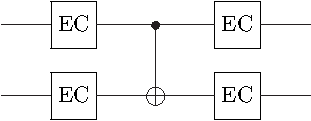
\includegraphics[width=.75\textwidth]{cnotExRec}};}
\end{tikzpicture}
}

\begin{tikzpicture}[overlay]
\node[coordinate] at(exRec) {exRec};
\node[yshift=.3cm,coordinate] (ll) at(exRec) {X};
\node[xshift=9.8cm,coordinate] (lr) at(ll) {X};
\node[yshift=4.3cm,coordinate] (ul) {X};
% Errors
\redX[1cm][2.7cm]
\redX[1.55cm][2.5cm]
\redX[1.66cm][3cm]
\redX[3cm][2.5cm] 
\redX[1.5cm][.5cm] 
\redX[3cm][.7cm]
\redX[6.3cm][1cm]
\redX[6.8cm][.5cm] 
\redX[6.5cm][2.8cm]
\redX[8cm][1.3cm] 
\redX[1.4cm][1.2cm] 
\redX[4.5cm][.85cm]
\redX[8.3cm][2.5cm]
\redX[8.4cm][.45cm]


% Gridlines
\foreach \x in {.15\textwidth, .3\textwidth,  .5\textwidth, .65\textwidth}
  {
    \node[xshift=\x,coordinate] (a) at(ul){};
    \node[xshift=\x,coordinate] (b) at(ll){};
    \path[->] (a) edge[blue,ultra thick,-] (b);
  }
\foreach \y in {2cm}
  {
    \node[yshift=\y,coordinate] (a) at(ll){};
    \node[yshift=\y,coordinate] (b) at(lr){};
    \path[->] (a) edge[blue,ultra thick,-] (b);
  }
\end{tikzpicture}

\end{preview}

\end{document}


